\section{Hasil dan Pembahasan}

%=========================================================%
%               TULIS ISI PEMBAHASAN DI SINI              %
% Jangan Lupa untuk Menghapus Contoh Tulisan di Bawah Ini %
%=========================================================%

Metode Jaringan Saraf Tiruan (JST) adalah pemrosesan informasi yang terinspirasi oleh sistem saraf biologi. JST mampu mengenali kegiatan dengan berbasis data pada masa lalu. Data masa lalu akan dipelajari oleh JST sehingga mempunyai kemampuan untuk memberi keputusan terhadap data yang belum pernah dipelajari \cite{Hasanah-2014:isoss}.

\subsection{\textit{Backpropagation}}

\textit{Backpropagation} merupakan algoritma pembelajaran terawasi yang terdiri dari lapisan \textit{input}, lapisan tersembunyi, dan \textit{output} dengan mengubah bobot-bobot yang terhubung pada masing-masing lapisan \cite{shi-2012}.

\begin{figure}[H]
    \centering
    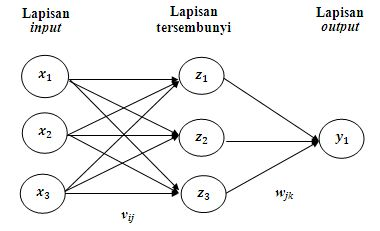
\includegraphics[width=.6\linewidth]{image/JST.jpg}
    \caption{Jaringan Saraf Tiruan}
    \label{fig:jaringan-saraf-tiruan}
    \figuresource{\citeA{raymundo-2012:artificial}}
\end{figure}

\autoref{fig:jaringan-saraf-tiruan} di atas merupakan contoh arsitektur JST \textit{Backpropagation} yang menunjukkan bahwa $x_1,\, x_2,\, x_3$ merupakan lapisan \textit{input}, $z_1,\, z_2,\, z_3$ merupakan lapisan tersembunyi, sedangkan $y_1$ merupakan lapisan \textit{output}. Antara lapisan \textit{input} ke lapisan tersembunyi dihubungkan oleh masing-masing bobot sama halnya antara lapisan tersembunyi ke lapisan \textit{output} dihubungkan oleh masing-masing bobot. Setiap lapisan \textit{input}, bobot, dan lapisan tersembunyi didapatkan dengan melakukan simulasi --- diharapkan menghasilkan nilai \textit{error} dalam hal ini yaitu kuadrat tengah galat (KTG) minimum.

\noindent Model JST \textit{Backpropagation} adalah sebagai berikut:

\begin{equation}
    y_k = f_k \left( \sum_{j = 1}^{p} w_{jk} f_j \left( v_{0j} + \sum_{i = 1}^{n} x_i v_{ij} \right) + w_{0k} \right)  \label{eq1}
\end{equation}

\begin{tabbing}
    $w_{0k}$ \= = bobot bias pada unit \textit{output} $y_k$ \\
    $v_{0j}$ \> = bobot bias pada unit tersembunyi $z_j$ \\
    $v_{ij}$ \> = bobot garis dari unit $x_1$ ke unit tersembunyi $z_j$ \\
    $w_{jk}$ \> = bobot garis dari $z_j$ ke unit \textit{output} $y_k$ \\
    $f_k$ \> = fungsi aktivasi pada unit tersembunyi ke \textit{output} \\
    $f_j$ \> = fungsi aktivasi pada unit \textit{input} ke tersembunyi \\
    $x_1$ \> = unit \textit{input} ke-$i$ \\
    $z_j$ \> = unit tersembunyi ke-$j$ \\
    $y_k$ \> = unit \textit{output} ke-$k$ \\
    $i$ \> = $1,\, \dots,\, n$ \\
    $j$ \> = $1,\, \dots,\, p$ \\
    $k$ \> = $1,\, \dots,\, l$ \\
    $k$ \> = banyaknya unit \textit{input} \\
    $p$ \> = banyaknya unit tersembunyi \\
    $l$ \> = banyaknya unit \textit{output}
\end{tabbing}

\subsection{Normalisasi}

Normalisasi digunakan untuk melihat hasil \textit{output} pada JST \textit{Backpropagation} berada pada nilai 0 sampai dengan 1. Normalisasi dapat menghasilkan ketepatan klasifikasi yang cukup tinggi pada status mahasiswa prodi Statistika UT \cite{aksu-2019:effect}, dengan menggunakan rumus sebagai berikut:

\begin{equation}
    x = \frac{0{,}8(x - a)}{b - a} + 0{,}1  \label{eq2}
\end{equation}

\subsection{Fungsi Aktivasi}

Fungsi aktivasi merupakan suatu fungsi yang digunakan untuk membawa nilai  \textit{input} menuju \textit{output} yang diinginkan. Fungsi ini harus memenuhi beberapa syarat yaitu kontinu, terdiferensial dengan mudah, dan fungsi yang tidak turun. Fungsi aktivasi yang digunakan dalam JST \textit{Backpropagation} yaitu fungsi sigmoid biner, fungsi tangen sigmoid, dan fungsi linear \cite{mirtalaei-2012:trust}.

\subsection{Hasil Eksplorasi Data}

Berikut ini merupakan hasil eksplorasi data yang menggambarkan status mahasiswa prodi Statistika UT berdasarkan jenis kelamin, kelompok usia, pendidikan, status pernikahan, dan status pekerjaan.

\begin{table}[H]
    \centering
    \caption{Status Mahasiswa Berdasarkan Jenis Kelamin}
    \label{table:status-jenis-kelamin}
    \begin{tblr}{colspec={l c c}, row{1,2}={font=\bfseries}, hline{1-3,Z}={1-Z}{solid}, colsep=14pt}
        \SetCell[r=2]{valign=m} Jenis Kelamin & \SetCell[c=2]{} Persentase (\%) & \\
        & Tidak Aktif & Aktif \\
        Pria & 35,9 & 64,1 \\
        Wanita & 29,1 & 70,9
    \end{tblr}
\end{table}

Berdasarkan \autoref{table:status-jenis-kelamin} di atas menunjukkan bahwa persentase wanita yang aktif sebagai mahasiswa UT prodi Statistika yaitu sebesar 70,9\%. Persentase tersebut lebih besar bila dibandingkan dengan pria yaitu sebesar 64,1\%. Maka dapat disimpulkan wanita lebih mendominasi mengambil program studi Statistika dibandingkan dengan pria.

\begin{table}[H]
    \centering
    \caption{Status Mahasiswa Berdasarkan Kelompok Usia}
    \label{table:status-usia}
    \begin{tblr}{colspec={l c c}, row{1,2}={font=\bfseries}, hline{1-3,Z}={1-Z}{solid}, colsep=14pt}
        \SetCell[r=2]{valign=m} Kelompok Usia & \SetCell[c=2]{} Status Mahasiswa (\%) & \\
        & Tidak Aktif & Aktif \\
        $\leq 25$ & 8,5 & 91,5 \\
        26 -- 35 & 39,1 & 60,9 \\
        36 -- 45 & 48,8 & 51,2 \\
        46 -- 55 & 44,1 & 55,9 \\
        $\geq 56$ & 40 & 60
    \end{tblr}
\end{table}

\autoref{table:status-usia} di atas menunjukkan bahwa persentase yang paling besar sebagai mahasiswa aktif yaitu pada kelompok usia $\leq 25$ tahun sebesar 91,5\%, diikuti pada kelompok usia 26--35 tahun, $\geq 56$ tahun, 46--55 tahun, dan 36--45 tahun. Maka dapat disimpulkan kelompok usia $\leq 25$ tahun adalah mahasiswa yang paling banyak mengambil prodi Statistika karena pada usia tersebut merupakan mahasiswa \textit{fresh graduate} dari sekolah menengah ke atas.

\begin{table}[H]
    \centering
    \caption{Status Mahasiswa Berdasarkan Pendidikan}
    \label{table:status-pendidikan}
    \begin{tblr}{colspec={l c c}, row{1,2}={font=\bfseries}, hline{1-3,Z}={1-Z}{solid}, colsep=14pt}
        \SetCell[r=2]{valign=m} Pendidikan & \SetCell[c=2]{} Status Mahasiswa (\%) & \\
        & Tidak Aktif & Aktif \\
        SLTA & 31,9 & 68,1 \\
        Diploma & 35,9 & 64,1 \\
        S1 & 29 & 71 \\
        S2 & 0 & 100 \\
        S3 & 100 & 0
    \end{tblr}
\end{table}

\autoref{table:status-pendidikan} menunjukkan bahwa persentase pendidikan S2 dan S1 yang berstatus aktif sebagai mahasiswa UT prodi Statistika yaitu S2 100\% dan S1 70\%. Hal in dapat disimpulkan bahwa status mahasiswa aktif yang telah berpendidikan S1 dan S2 lebih mudah mengikuti perkuliahan di prodi Statistika karena telah mempelajari statistika pada saat mengikuti perkuliahan sebelumnya dan mengambil statistika lagi sebagai penunjang untuk meningkatkan kompetensi dalam hal analisis dan pengolahan data. Sedangkan yang berpendidikan S3 tidak aktif 100\%. Setelah dilakukan analisis diketahui bahwa hanya terdapat satu mahasiswa S3 saja yang pada saat itu sedang tidak aktif menjadi mahasiswa.

\begin{table}[H]
    \centering
    \caption{Status Mahasiswa Menurut Status Pernikahan}
    \label{table:status-pernikahan}
    \begin{tblr}{colspec={l c c}, row{1,2}={font=\bfseries}, hline{1-3,Z}={1-Z}{solid}, colsep=14pt}
        \SetCell[r=2]{valign=m} Status Pernikahan & \SetCell[c=2]{} Status Mahasiswa (\%) & \\
        & Tidak Aktif & Aktif \\
        Belum Menikah & 26,1 & 73,9 \\
        Menikah & 38 & 62
    \end{tblr}
\end{table}

\autoref{table:status-pernikahan} di atas menunjukkan bahwa persentase mahasiswa aktif yang berdasarkan status pernikahan diketahui bahwa mahasiswa yang belum menikah pada prodi Statistika yaitu sebesar 73,9\%. Hal ini menunjukkan bahwa mahasiswa yang belum menikah lebih mudah mengikuti proses perkuliahan di UT pada prodi Statistika.

\begin{table}[H]
    \centering
    \caption{Status Mahasiswa Berdasarkan Status Pekerjaan}
    \label{table:status-pekerjaan}
    \begin{tblr}{colspec={l c c}, row{1,2}={font=\bfseries}, hline{1-3,Z}={1-Z}{solid}, colsep=14pt}
        \SetCell[r=2]{valign=m} Status Pernikahan & \SetCell[c=2]{} Status Mahasiswa (\%) & \\
        & Tidak Aktif & Aktif \\
        Tidak Bekerja & 27 & 73 \\
        Karyawan Swasta & 30,5 & 69,5 \\
        Wiraswasta & 26,4 & 73,6 \\
        PNS & 41,2 & 58,8 \\
        TNI/Polri & 100 & 0
    \end{tblr}
\end{table}

\autoref{table:status-pekerjaan} di atas menunjukkan bahwa mahasiswa aktif di prodi Statistika adalah mahasiswa yang bekerja sebagai wiraswasta sebesar 73,6\% dan tidak bekerja sebesar 73\%. Hal ini menunjukkan bahwa mahasiswa yang bekerja sebagai wiraswasta dan yang tidak bekerja lebih mudah mengikuti proses perkuliahan di prodi Statistika.

\subsection{Simulasi JST \textit{Backpropagation}}

Selanjutnya dilakukan pengklasifikasian untuk status mahasiswa prodi Statistika dengan menggunakan metode Jaringan Saraf Tiruan (JST) \textit{Backpropagation}. Simulasi dilakukan dengan memaksimalkan fungsi aktivasi dan \textit{learning rate} ($\alpha$), maka model JST \textit{Backpropagation} pada data \textit{training} yang terbentuk pada unit lapisan \textit{input} yaitu 15 unit, lapisan unit \textit{output} 1, dan 8 lapisan unit tersembunyi. Hasil simulasi dapat dilihat pada \autoref{table:hasil-simulasi-fungsi-n-alpha} di bawah ini.

\begin{table}[H]
    \centering
    \caption{Hasil Simulasi Fungsi Aktivasi dan \textit{Learning Rate}}
    \label{table:hasil-simulasi-fungsi-n-alpha}
    \begin{tblr}{
            colspec={c l l c l c c l l c l}, 
            hline{1,2,Z}={1-5,7-Z}{solid}, 
            row{1}={font=\bfseries, halign=c, valign=m}
            }
        No. & \SetCell[c=2]{} {Fungsi \\ Aktivasi} && {\textit{Learning} \\ \textit{Rate} ($\alpha$)} & KTG && No. & \SetCell[c=2]{} {Fungsi \\ Aktivasi} && {\textit{Learning} \\ \textit{Rate} ($\alpha$)} & KTG \\
        1 & Log & Linear & 0,01 & 0,015002 && 11 & Log & Linear & 0,5 & 0,013088 \\
        2 & Tan & Linear & 0,01 & 0,014702 & & 12 & Tan & Linear & 0,5 & 0,013705 \\
        3 & Log & Linear & 0,1 & 0,013049 & & 13 & Log & Linear & 0,6 & 0,016399 \\
        4 & Tan & Linear & 0,1 & 0,007924 & & 14 & Tan & Linear & 0,6 & 0,010384 \\
        5 & Log & Linear & 0,2 & 0,014674 & & 15 & Log & Linear & 0,7 & 0,012494 \\
        6 & Tan & Linear & 0,2 & 0,013854 & & 16 & Tan & Linear & 0,7 & 0,010625 \\
        7 & Log & Linear & 0,3 & 0,013561 & & 17 & Log & Linear & 0,8 & 0,014627 \\
        8 & Tan & Linear & 0,3 & 0,012849 & & 18 & Tan & Linear & 0,8 & 0,005195 \\
        9 & Log & Linear & 0,4 & 0,014409 & & 19 & Log & Linear & 0,9 & 0,012066 \\
        10 & Tan & Linear & 0,4 & 0,014921 & & 20 & Tan & Linear & 0,9 & 0,013741
    \end{tblr}
\end{table}

Berdasarkan \autoref{table:hasil-simulasi-fungsi-n-alpha} menunjukkan bahwa fungsi aktivasi tangen sigmoid pada lapisan \textit{input} ke lapisan tersembunyi dan linear pada lapisan tersembunyi ke lapisan \textit{output} serta \textit{learning rate} 0,8 menghasilkan nilai KTG yang minimum, yaitu sebesar 0,005195. Maka berdasarkan hasil simulasi yang telah dilakukan pada model JST \textit{Backpropagation} adalah sebagai berikut:

\begin{equation}
    y_k = f_k \left(\sum_{j = 1}^{8} w_{jk} f_j \left(v_{0j} + \sum_{i = 1}^{15} x_i v_{ij} \right) + w_{0k}\right)  \label{eq:3}
\end{equation}

Jumlah 15 unit \textit{input} terdiri dari jenis kelamin, usia, pendidikan (SLTA/SMK, Diploma, S1, S2), status pernikahan, status pekerjaan (tidak bekerja, karyawan swasta, wiraswasta, PNS), tahun registrasi awal, jumlah registrasi, SKS tempuh, dan IPK.

\begin{figure}[H]
    \centering
    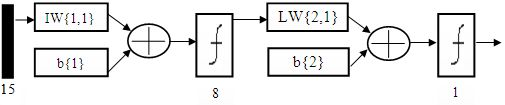
\includegraphics[width=.6\linewidth]{image/Hasil Simulasi JSTB.jpg}
    \caption{Hasil Simulasi Jaringan Saraf Tiruan \textit{Backpropagation}}
    \label{fig:hasil-simulasi-jstb}
\end{figure}

\autoref{fig:hasil-simulasi-jstb} menunjukkan bahwa simulasi yang telah didapatkan dengan 15 unit lapisan \textit{input}, 8 unit lapisan tersembunyi, 1 unit lapisan \textit{output}, IW\{1,1\} dan b\{1\} adalah bobot, bias akhir yang terdapat pada lapisan \textit{input} ke lapisan tersembunyi, LW\{2,1\} dan b\{2\} adalah bobot, bias akhir yang terdapat pada lapisan tersembunyi ke lapisan \textit{output}.

Hasil \textit{output} pada JST \textit{Backpropagation} dilakukan analisis lanjutan dengan menggunakan kurva ROC sebagai berikut:

\begin{figure}[H]
    \centering
    \hspace{-1.24cm}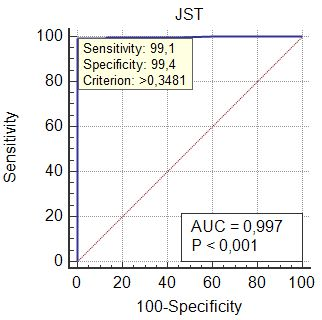
\includegraphics[width=.5\linewidth]{image/Kurva ROC Data Training.jpg}
    \caption{Kurva ROC Data \textit{Training}}
    \label{fig:kurva-roc-dataTraining}
\end{figure}

Pada \autoref{fig:kurva-roc-dataTraining} didapatkan hasil klasifikasi terbaik pada data \textit{training}, yaitu pada saat \textit{cut-off point} beada di nilai 0,3481. Sehingga didapatkan nilai sensitivitas sebesar 99,1\% dan spesifisitas 99,4\%. Di \autoref{table:hasil-jst-dataTraining} ini merupakan hasil tabulasi silang antara kelas \textit{output} dan data \textit{training} dengan hasil klasifikasi menggunakan metode JST \textit{Backpropagation} adalah sebagai berikut:

\begin{table}[H]
    \centering
    \caption{Hasil JST Data \textit{Training}}
    \label{table:hasil-jst-dataTraining}
    \begin{tblr}{colspec={l c c}, row{1,2}={font=\bfseries}, hline{1-3,Z}={1-Z}{solid}, colsep=14pt}
        \SetCell[r=2]{valign=m} Kelas & \SetCell[c=2]{} Hasil JST (\%) & \\
        & Tidak Aktif & Aktif \\
        Tidak Aktif & 99,43 & 0,57 \\
        Aktif & 0,86 & 99,14
    \end{tblr}
\end{table}

Berdasarkan \autoref{table:hasil-jst-dataTraining}, didapatkan bahwa ketepatan JST \textit{Backpropagation} dalam klasifikasi data \textit{training} untuk mahasiswa tidak aktif sebesar 99,43\% dan mahasiswa aktif sebesar 99,14\%, sehingga dapat disimpulkan bahwa metode JST \textit{Backpropagation} cukup baik digunakan untuk klasifikasi data \textit{training} pada status mahasiswa prodi Statistika Universitas Terbuka.

Nilai bobot dan bias yang didapatkan pada proses data \textit{training} digunakan untuk validasi data \textit{testing} dengan menggunakan \textit{cut-off point} sebesar 0,3481 maka didapatkan hasil ketepatan klasifikasi data \textit{testing} pada \autoref{table:hasil-jst-dataTesting} berikut ini.

\begin{table}[H]
    \centering
    \caption{Hasil JST Data \textit{Testing}}
    \label{table:hasil-jst-dataTesting}
    \begin{tblr}{colspec={l c c}, row{1,2}={font=\bfseries}, hline{1-3,Z}={1-Z}{solid}, colsep=14pt}
        \SetCell[r=2]{valign=m} Kelas & \SetCell[c=2]{} Hasil JST (\%) & \\
        & Tidak Aktif & Aktif \\
        Tidak Aktif & 94 & 6 \\
        Aktif & 6,06 & 93,94
    \end{tblr}
\end{table}

Berdasarkan \autoref{table:hasil-jst-dataTesting}, didapatkan bahwa ketepatan JST \textit{Backpropagation} dalam klasifikasi data \textit{testing} untuk mahasiswa tidak aktif sebesar 94\% dan yang aktif tepat sebesar 93,94\%, sehingga dapat disimpulkan bahwa metode JST \textit{Backpropagation} cukup baik untuk klasifikasi data \textit{testing} pada status mahasiswa prodi Statistika UT.